%%
%% This is file `sample-sigconf.tex',
%% generated with the docstrip utility.
%%
%% The original source files were:
%%
%% samples.dtx  (with options: `sigconf')
%% 
%% IMPORTANT NOTICE:
%% 
%% For the copyright see the source file.
%% 
%% Any modified versions of this file must be renamed
%% with new filenames distinct from sample-sigconf.tex.
%% 
%% For distribution of the original source see the terms
%% for copying and modification in the file samples.dtx.
%% 
%% This generated file may be distributed as long as the
%% original source files, as listed above, are part of the
%% same distribution. (The sources need not necessarily be
%% in the same archive or directory.)
%%
%% The first command in your LaTeX source must be the \documentclass command.
\documentclass[sigconf]{acmart}

%%
%% \BibTeX command to typeset BibTeX logo in the docs
\AtBeginDocument{%
  \providecommand\BibTeX{{%
    \normalfont B\kern-0.5em{\scshape i\kern-0.25em b}\kern-0.8em\TeX}}}

%% Rights management information.  This information is sent to you
%% when you complete the rights form.  These commands have SAMPLE
%% values in them; it is your responsibility as an author to replace
%% the commands and values with those provided to you when you
%% complete the rights form.
\setcopyright{acmcopyright}
\copyrightyear{2020}
\acmYear{2020}
\acmDOI{10.1145/1122445.1122456}

%% These commands are for a PROCEEDINGS abstract or paper.
\acmConference[SBES '20]{SBES '2020: XXXIV BRAZILIAN SYMPOSIUM ON SOFTWARE ENGINEERING (SBES 2020)}{October 19--23, 2020}{Natal, Brazil}
\acmBooktitle{XXXIV BRAZILIAN SYMPOSIUM ON
SOFTWARE ENGINEERING (SBES 2020),
  October 19--23, 2020, Natal, Brazil}


%%
%% Submission ID.
%% Use this when submitting an article to a sponsored event. You'll
%% receive a unique submission ID from the organizers
%% of the event, and this ID should be used as the parameter to this command.
%%\acmSubmissionID{123-A56-BU3}

%%
%% The majority of ACM publications use numbered citations and
%% references.  The command \citestyle{authoryear} switches to the
%% "author year" style.
%%
%% If you are preparing content for an event
%% sponsored by ACM SIGGRAPH, you must use the "author year" style of
%% citations and references.
%% Uncommenting
%% the next command will enable that style.
%%\citestyle{acmauthoryear}

%%
%% end of the preamble, start of the body of the document source.
\begin{document}

%%
%% The "title" command has an optional parameter,
%% allowing the author to define a "short title" to be used in page headers.
\title{CoNCRA: A Convolution Network Code Retrieval Approach}

%%
%% The "author" command and its associated commands are used to define
%% the authors and their affiliations.
%% Of note is the shared affiliation of the first two authors, and the
%% "authornote" and "authornotemark" commands
%% used to denote shared contribution to the research.
\author{Marcelo de Rezende Martins}
\email{rezende.martins@gmail.com}
\affiliation{%
  \institution{IPT – Institute for Technological Research}
  \city{Sao Paulo}
  \state{Sao Paulo}
  \country{Brazil}
}


\author{Marco Aurélio Gerosa}
\email{marco.gerosa@nau.edu}
\affiliation{%
  \institution{Northern Arizona University (NAU)}
  \city{Flagstaff}
  \state{Arizona}
  \country{United States}
}

%%
%% By default, the full list of authors will be used in the page
%% headers. Often, this list is too long, and will overlap
%% other information printed in the page headers. This command allows
%% the author to define a more concise list
%% of authors' names for this purpose.


%%
%% The abstract is a short summary of the work to be presented in the
%% article.
\begin{abstract}
   Code search is a prevalent task in software development process. According to \cite{what-developers-search-for-on-the-web:xia:2017}, developers spend 15\% of their time searching for API's examples, what a code does and how to fix a bug. A research at Google showed that developers search for code 12 times a day, checking 2 and 3 results per search session. Most of the time, they are looking for code examples \citep{sadowski-how-developers-search-for-code-case-study:2015}. Thus, improve the way developers find a code its an important productivity tool. In our work, we present a novel approach to retrieve code semantically using a convolution neural network. Our preliminary results showed a prominent technique which improved the state of art \citep{cambronero-deep-code-search-2019} by 5\% on the average and it could retrieve the most relevant code snippets for a natural language query in the first 3 (three) positions by 80\% of the time. 
\end{abstract}

%%
%% The code below is generated by the tool at http://dl.acm.org/ccs.cfm.
%% Please copy and paste the code instead of the example below.
%%
\begin{CCSXML}
<ccs2012>
   <concept>
       <concept_id>10010147.10010257.10010293.10010319</concept_id>
       <concept_desc>Computing methodologies~Learning latent representations</concept_desc>
       <concept_significance>300</concept_significance>
       </concept>
   <concept>
       <concept_id>10011007.10011074.10011092.10011096</concept_id>
       <concept_desc>Software and its engineering~Reusability</concept_desc>
       <concept_significance>300</concept_significance>
       </concept>
   <concept>
       <concept_id>10011007.10011006.10011008</concept_id>
       <concept_desc>Software and its engineering~General programming languages</concept_desc>
       <concept_significance>300</concept_significance>
       </concept>
 </ccs2012>
\end{CCSXML}

\ccsdesc[300]{Computing methodologies~Learning latent representations}
\ccsdesc[300]{Software and its engineering~Reusability}
\ccsdesc[300]{Software and its engineering~General programming languages}


%%
%% Keywords. The author(s) should pick words that accurately describe
%% the work being presented. Separate the keywords with commas.
\keywords{code search, neural networks, joint embedding}

%% A "teaser" image appears between the author and affiliation
%% information and the body of the document, and typically spans the
%% page.
\begin{teaserfigure}
  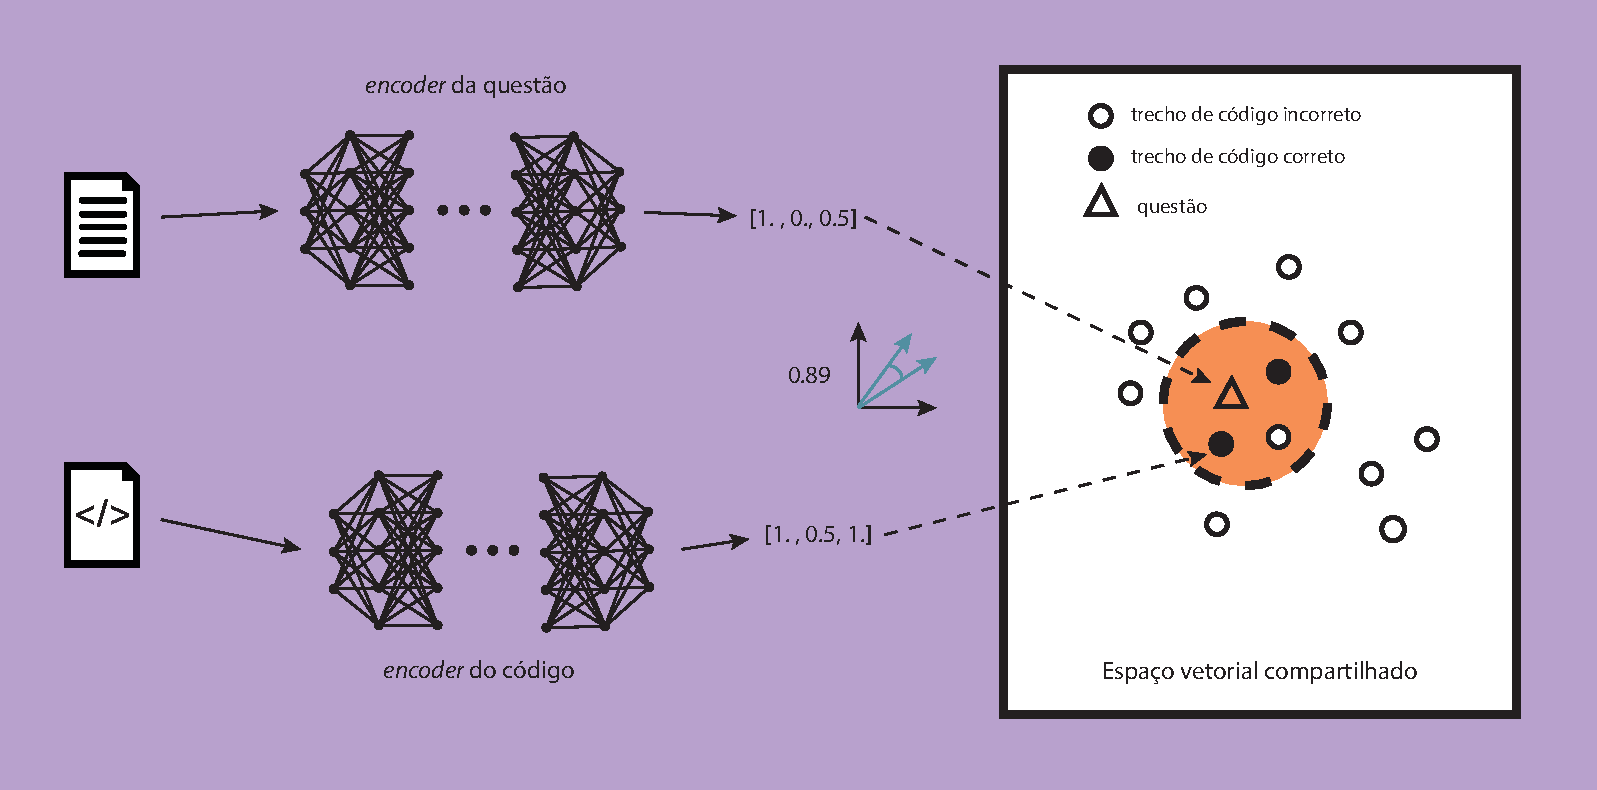
\includegraphics[width=\textwidth]{figuras/joint_embedding.pdf}
  \caption{Illustration of \emph{joint embedding} technique for code retrieval. Two neural networks map a question and a code snippet into a common vector space. The distance between the vectors reflects the relevance of a code snippet to a question.}
  \Description{None}
  \label{fig:joint-embedding}
\end{teaserfigure}

%%
%% This command processes the author and affiliation and title
%% information and builds the first part of the formatted document.
\maketitle

\section{Introduction}

The advent of open source code and open question answering sites related to programming contributed to improve the way developers code today. Nowadays, code search is a daily routine task at software development process. Developers spend 15\% of their time searching for how a code works, a bug fix and API's usage \cite{what-developers-search-for-on-the-web:xia:2017}. According to \cite{sadowski-how-developers-search-for-code-case-study:2015}, developers at Google search for code 12 times a day, clicking on 2 to 3 results by average per search session. Most of them are looking for code examples. Thus, improve the way developers find a code it's an important productivity tool.  

Most of developers use general purpose search engine (GPSE) to look for code (e.g. Google). GPSE uses page rank and other indexes tactics that are not optimized for searching code. Then, GPSE are not capable of finding a code semantically, unless a code has a accompanying description. According to ZZZ, developers spend more time, visit more pages and change a query more times when they are searching for code compared to non-code related search.

GitHub, a popular open source code repository, have tried to build a semantic code search. They extracted millions of lines of code from his repositories and matched each code with a dosctring. The final results weren't satisfactory, the tool could find a relevant code only if the query matches the docstring description (cite HHHHHH). According to XXXXX, a user's intent were better matched with questions extracted from open question-answering sites related to programming, e.g., StackOverflow. Those sites permit users to ask a question and check the best answer for him. Other users can vote for the most helpful answer and mark wrong or not helpful ones. Those collective actions help to curate and organize information, creating a valuable repository.

There are a lot of works about semantic code search (UUUUUU). The first ones were based on deductive-logic rules and manual feature extraction from code. The recent success of artificial neural networks, due to Big Data and computational resources available, shifted works to machine learning based approach. ZZZZZ also coined a name, neural code search, i.e., code search based on neural networks.

Most of works applied neural networks to summarize and retrieve code snippets. Code summarization and retrieval are two different activities, each one with it's metric and trait. We are proposing an novel approach for code retrieval. Different from other works, which presented an neural network with attention mechanism and a recurrent neural network (RRRR, GGGG), we are proposing a code retrieval based on convolution networks. ZZZ and YYY paired code snippets and docstring, we matched code with questions extracted from StackOverflow.

\subsection{Contributions of this work}

We can summarize the shortcomings of the existing work:
most of neural networks approaches summarize and retrieve a code, although each one has its idiosyncrasy. As far as we know, we are the first to apply convolutional neural network to code retrieval, due to good results in answer selection tasks (TTTTTT). Most of works paired code and docstring, even though docstring doesn't match user's intent. Our research are trying to address each of these in turn by proposing and analyzing the CoNCRA, \emph{a Convolution Network Code Retrieval Approach}.

\begin{itemize}
    \item We are proposing the CoNCRA, which is motivated
by the good results of convolution networks at Natutal Language Processing (NLP) tasks. 
    \item We paired code and questions collected from StackOverflow, based on a public available dataset (YYYY).

    \item We evaluated the efficacy of our approach against two other proposals.
    
\end{itemize}







\section{Methodology}

According to \cite{cambronero-deep-code-search-2019}, the main goal of code retrieval is:

\emph{Retrieve code snippets from a code corpus that most closely match a developer's intent, which is expressed in natural language.}

The first proposals for code search used tools based on deductive-logic rules and manual feature extraction. Deductive-logic approach, e.g. boolean model, finds a code that matches exactly the keywords expressed in the query. According to ZZZ, those approaches are good at finding API's call and error's message, but it struggles to find reusable code and examples that don't have a exactly match between the code and query. Thus, there is a need to look for a semantic code search.

Neural networks showed good results at translation, question-answering and classifications tasks in NLP, it could infer words semantic and phrases context. Then, most of recent works adopted neural networks approach. Cambronero coined a term, \emph{neural code search}, searching for code using neural networks.

The marjority of works adopted the same strategy, which is to discriminate relevant code snippets from non-relevant one's based on an user's intent. In pursuance of that, code retrieval are reduced to a ranking problem where neural networks should be able to place code snippets that closely match developer's intent in the first rank. The most common strategy to do this is \emph{joint embedding}. Joint embedding maps heterogeneous data into a common vector space, where the distance between embedded input reflects the similarity between the underlying items \cite{li-joint-embedding-images-2015} (see Figure~\ref{fig:joint-embedding}).

In order to apply joint embedding, 3 (three) items had to be considered:

\begin{itemize}
    \item Word embedding
    \item Sentence embedding
    \item Joint embedding
\end{itemize}

Embedding refers to a continuous vector in a lower dimensional vector space. A function that maps an input to a continuous vector is called \emph{encoder}. So, given an input set $X$, an encoder function $F$ can be defined as \cite{cambronero-deep-code-search-2019}:

\begin{equation}
    F: X \to E
\end{equation}

In our case, $X$ can be a question or code snippet and $E$ is a set of continuous vectors or embeddings, such that $E \subset R^{d}$, where $d$ is the dimension. Our objective is to learn two encoders $F$ and $G$ that maps a question and a code snippet, respectively, into a common vector space, so that the distance between the vectors reflect the relevance of a code snippet to a question (see Figure~\ref{fig:joint-embedding}). Our CoNCRA approach applies a convolution network to learn the sentence embedding, but in order to do that, we also had to define how words had been mapped and how the questions and code snippets embedded vectors are jointly grouped.

\subsection{Word embedding}

\subsection{Sentence embedding}

\subsection{Joint embedding}



\section{Experiment and Results}

\subsection{Threats to validity}

\section{Related Work}

\section{Conclusion}

\section{Acknowledgments}

Identification of funding sources and other support, and thanks to
individuals and groups that assisted in the research and the
preparation of the work should be included in an acknowledgment
section, which is placed just before the reference section in your
document.

This section has a special environment:
\begin{verbatim}
  \begin{acks}
  ...
  \end{acks}
\end{verbatim}
so that the information contained therein can be more easily collected
during the article metadata extraction phase, and to ensure
consistency in the spelling of the section heading.

Authors should not prepare this section as a numbered or unnumbered {\verb|\section|}; please use the ``{\verb|acks|}'' environment.

\section{Appendices}

If your work needs an appendix, add it before the
``\verb|\end{document}|'' command at the conclusion of your source
document.

Start the appendix with the ``\verb|appendix|'' command:
\begin{verbatim}
  \appendix
\end{verbatim}
and note that in the appendix, sections are lettered, not
numbered. This document has two appendices, demonstrating the section
and subsection identification method.

\section{SIGCHI Extended Abstracts}

The ``\verb|sigchi-a|'' template style (available only in \LaTeX\ and
not in Word) produces a landscape-orientation formatted article, with
a wide left margin. Three environments are available for use with the
``\verb|sigchi-a|'' template style, and produce formatted output in
the margin:
\begin{itemize}
\item {\verb|sidebar|}:  Place formatted text in the margin.
\item {\verb|marginfigure|}: Place a figure in the margin.
\item {\verb|margintable|}: Place a table in the margin.
\end{itemize}

%%
%% The acknowledgments section is defined using the "acks" environment
%% (and NOT an unnumbered section). This ensures the proper
%% identification of the section in the article metadata, and the
%% consistent spelling of the heading.
\begin{acks}
To Robert, for the bagels and explaining CMYK and color spaces.
\end{acks}

%%
%% The next two lines define the bibliography style to be used, and
%% the bibliography file.
\bibliographystyle{ACM-Reference-Format}
\bibliography{sample-base}

%%
%% If your work has an appendix, this is the place to put it.
\appendix

\section{Research Methods}

\subsection{Part One}

Lorem ipsum dolor sit amet, consectetur adipiscing elit. Morbi
malesuada, quam in pulvinar varius, metus nunc fermentum urna, id
sollicitudin purus odio sit amet enim. Aliquam ullamcorper eu ipsum
vel mollis. Curabitur quis dictum nisl. Phasellus vel semper risus, et
lacinia dolor. Integer ultricies commodo sem nec semper.

\subsection{Part Two}

Etiam commodo feugiat nisl pulvinar pellentesque. Etiam auctor sodales
ligula, non varius nibh pulvinar semper. Suspendisse nec lectus non
ipsum convallis congue hendrerit vitae sapien. Donec at laoreet
eros. Vivamus non purus placerat, scelerisque diam eu, cursus
ante. Etiam aliquam tortor auctor efficitur mattis.

\section{Online Resources}

Nam id fermentum dui. Suspendisse sagittis tortor a nulla mollis, in
pulvinar ex pretium. Sed interdum orci quis metus euismod, et sagittis
enim maximus. Vestibulum gravida massa ut felis suscipit
congue. Quisque mattis elit a risus ultrices commodo venenatis eget
dui. Etiam sagittis eleifend elementum.

Nam interdum magna at lectus dignissim, ac dignissim lorem
rhoncus. Maecenas eu arcu ac neque placerat aliquam. Nunc pulvinar
massa et mattis lacinia.

\end{document}
\endinput
%%
%% End of file `sample-sigconf.tex'.
